\chapter{Аналитическая часть}

\section{Описание словаря}

В данной лабораторной работе использовался словарь VR-игр.
Ключами в данном словаре были названия игр.
Значениями были объекты, которые имели характеристики данной игры, а именно:

\begin{itemize}
	\item Издатель;
	\item Год издания;
	\item Жанр;
	\item Возрастное ограничение;
	\item Цена.
\end{itemize}

\section{Теоретические данные}

Словари -- объекты, записанные парой "ключ-значение".
Отличным примером словаря является толковый словарь.
В данном словаре ключи -- это нужное нам слово, а значения --
это значение искомого слова. 
Ключи в словаре должны быть уникальными.

Поиск необходимой информации в словаре -- одна из фундаментальных
задач программирования.

\section{Поиск полным перебором}

Поиск полным перебором может производиться в неотсортированном словаре. 
Весь алгоритм сводится к последовательному прохождению 
по всему словарю и сравнению всех значений с ключом. 
Данный алгоритм имеет N + 1 случаев и
требует N сравнений для худшего случая.
Это простейший из алгоритмов поиска. 
Этот алгоритм не очень эффективен, однако 
он работает на произвольном списке.

\section{Бинарный поиск}

Бинарный поиск базируется на том, что словарь 
изначально отсортирован, что позволяет сравнивать
ключ с средним элементом, и, если, он меньше, то продолжать
искать в левой части, таким же методом, иначе в правой. 

На рис. \ref{ref:binSearch} показан пример бинарного поиска.

\begin{figure}[ht!]
	\centering{
		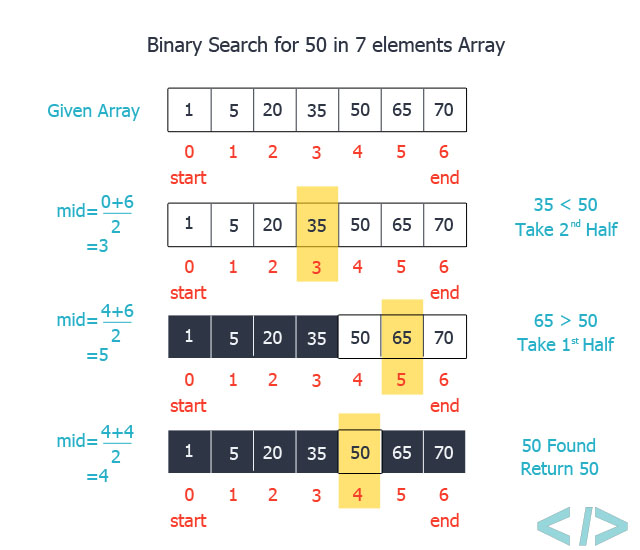
\includegraphics[width=0.8\textwidth]{Binary_Search.jpg}
		\caption{Бинарный поиск}
		\label{ref:binSearch}}
\end{figure}

\section{Частичный анализ}

Идея частичного анализа состоит в том, изначальный словарь
отсортирован по частоте первого символа. 
Также словарь имеет ключи равные буквам алфавита, а значениями 
являются словари с исходными данными, которые имеют первую букву схожую с ключом словаря.
На деле получается, что это простой толковый словарь, который имеет
в заголовке букву, а на странице все слова, которые начинаются на
написанную в заголовке букву. Поиск изначально осуществляется
по первой букве ключа. Далее, когда найден словарь, в котором
нужно искать искомое слово производится поиск полным перебором.


\section{Вывод}

В данном разделе были рассмотрены
основополагающие материалы, которые в дальнейшем потребуются
при реализации алгоритмов поиска в словаре.
